\documentclass[12pt]{article}
\usepackage{amssymb}
\usepackage{amsmath}
\usepackage{amsrefs}
\usepackage{graphicx}
\usepackage{bookman}
\usepackage{url}
\usepackage{amsthm}
\usepackage{verbatim}
\usepackage{xcolor}
\usepackage{setspace}
\usepackage{float}
\usepackage[margin=1in]{geometry}
\bibliographystyle{amsmath}
\doublespacing
\newtheorem{definition}{Definition}
\newtheorem{theorem}{Theorem}
\begin{document}

\title{Five Algorithms for Finding Matrix Solutions\\An Honors Project}
\author{Tyler Allen}
\date{}

\maketitle

\section{Introduction}

Systems of linear equations appear frequently in mathematics. Matrices have 
associated properties and algorithms that simplify handling systems of linear
equations dramatically. However, matrix equations become increasingly difficult to 
solve as the matrix increases in size. Thankfully, computers can perform these calculations
significantly faster than a human can by hand. I have implemented five different
algorithms for solving matrix equations: Gaussian Elimination, Gaussian Elimination with
Partial Pivoting, Jacobi's Method, The Gauss-Seidel Method, and a 
Successive Over-relaxation (SOR) Method. We will discuss the details of these 
algorithms and their implementation.



\section{General Implementation Information}
These algorithms for solving matrix equations  were implemented in Python 3.4, due to some improvements 
in Python's looping and printing methods over Python 2.7. It is likely that the
program will not execute succesfully or efficiently in Python 2.7. The implementation
provides a single interface for all of the provided methods, and uses command line 
arguments to accept the input. 

\begin{figure}[H]
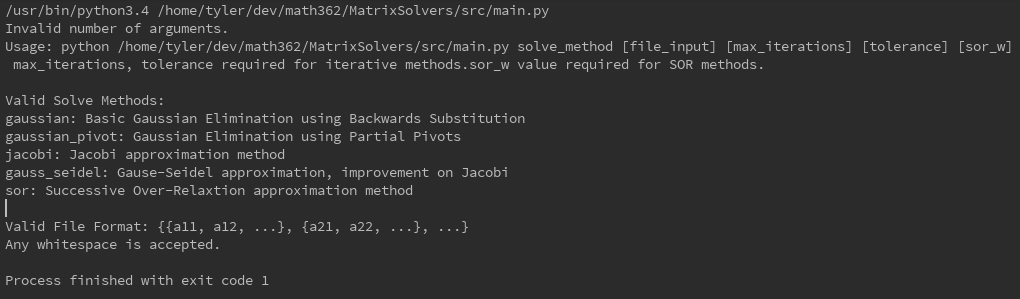
\includegraphics{usage.png}
\caption{The usage message printed in the event of incorrect arguments or missing files.}
\label{usage}
\end{figure}

Figure \ref{usage} contains a message shown to the user if a user inputs an incorrect
number of arguments or the file containing their matrix is unreadable or does not 
exist. Due to the complexity of matrix input, it was decided that using files for 
input would provide an easier experience to the user than allowing the user to 
enter the matrix at program execution.

\begin{figure}[H]
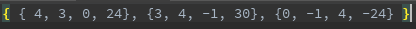
\includegraphics{input1.png}
\caption{An example input file.}
\label{input1}
\end{figure}
\begin{figure}[H]
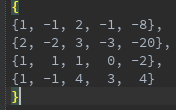
\includegraphics{input2.png}
\caption{Another example input file..}
\label{input2}
\end{figure}

Figures \ref{input1}, \ref{input2} show different formats for an input file. Some
test files are included with the source code. Any amount of whitespace may be used.
The matrix parsing algorithm is not advanced enough to detect most errors in user
input. A usage message will be displayed in the event that an input file contains
syntax errors. The matrix entry format is standard; outer brackets indicate the 
a matrix, inner brackets indicate a row, and commas seperate elements 
(values AND rows).  It was decided that this format is more flexible than entering
matrices directly into source code before executing the program, even with the
possibility of user error. The algorithms in the reference book specify $n x n$ 
matrices. The program will only function correctly when given an $n x n + 1$ 
matrix, where the additional vector is the $\bar{b}$ vector in $A\bar{x} = \bar{b}$.
This is because the algorithms expect the matrices to have single solutions,
$rank(n)$.
These implementations are also undefined in the event of inconsistency.

\section{Exact Methods}

Exact methods, such as Gaussian Elimination, give an exact solution. These 
exact solutions can be computationally expensive, but attempt to give solutions
without approximation. Some approximation is inherent due to computer roundoff
error. This error can be exaggerated greatly; a value with roundoff error 
will propogate the error throughout every calculation the value is involved in.
This can create exceedingly large error, but is a casualty of limited storage 
for floating point values. Some exact methods attempt to avoid this roundoff 
error.

\subsection{Gaussian Elimination with Backwards Substitution}
Gaussian Elimination is a standard method for solving matrix equations by-hand. If a 
matrix can be reduced to its Reduced Row Echelon form, the solution is easily
obtained. Each iteration of this method attempts to find a row to become the 
pivot row for the curret pivot column. This is done by finding the first non-zero
row. Once a pivot row and column are determined, the other values in that column
are eliminated using elementary row operations. 
This method can be accessed by using ``gaussian'' as the solution method
within the program.

\begin{figure}[H]
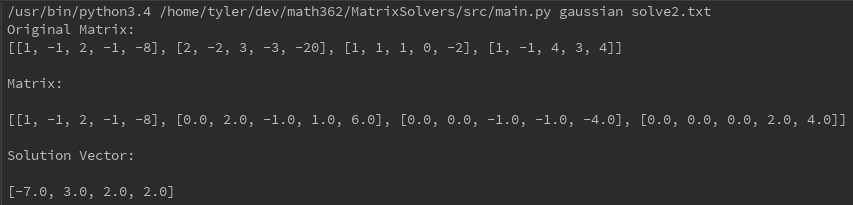
\includegraphics{gaussian.png}
\caption{Gaussian Elimination}
\label{gaussian}
\end{figure}

Figure \ref{gaussian} displays a usage of Gaussian Elimination. 


\subsection{Gaussian Elimination with Partial Pivoting}
Gaussian Elimination with Partial Pivoting was created to handle the 
computational roundoff error issue. The difference between Gaussian Elimination
with Backwards Substitution and this method is in the choice of pivot rows; 
rather than use the first available non-zero entry in the appropriate column
 as the pivot row, we use the entry in the pivot column with the highest magnitude (i.e. highest absolute value). 
 This will produce a more accurate result with less roundoff error. 

\begin{figure}[H]
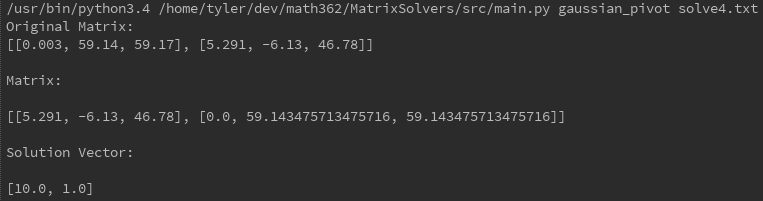
\includegraphics{pivot.png}
\caption{Gaussian Elimination with Partial Pivoting}
\label{pivot}
\end{figure}

\begin{figure}[H]
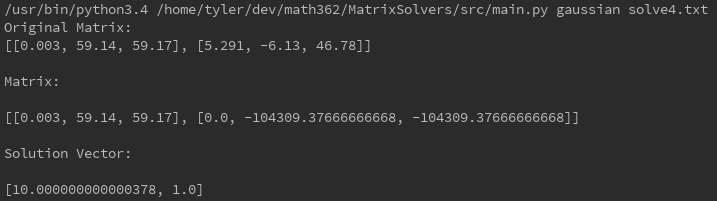
\includegraphics{badgaussian.png}
\caption{Gaussian Elimination}
\label{badgaussian}
\end{figure}

Figure \ref{pivot} displays one usage of this method. The same matrix equation is solved
using Gaussian Elimination with Backwards Substitution in Figure \ref{badgaussian}. 
The solution provided using the Partial Pivoting method provides a far more 
precise result. This method can be accessed by using ``gaussian\_pivot'' as the 
solution method within the program.


\section{Iterative Methods}
Iterative methods provide approximate solutions to matrix equations. For large
matrices, these methods are far more computationally efficient than their
exact counterparts. However, accuracy is lost without a sufficient number of 
iterations and a sufficiently lower tolerance. 

\subsection{Jacobi's Method}
Jacobi's method is one such approximate method. It requires a candidate solution
to be provided as a guess. This algorithm assumes the guess to be $\bar{0}$ in 
every case. Jacobi's method then uses the provided candidate to approach the 
actual solution. After an iteration, if the maximum number of iterations is exceeded
or the current solution's distance from the actual solution is within the tolerance 
level, we use the current solution. Otherwise, the current solution is the new 
candidate for the next iteration. 
\begin{figure}[H]
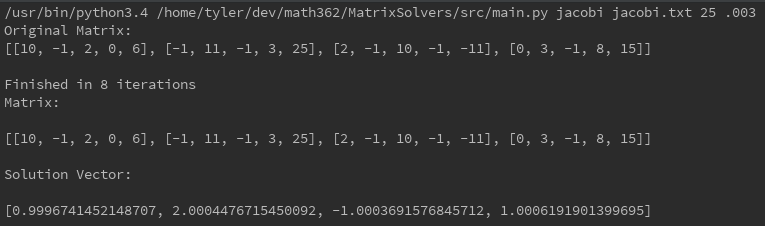
\includegraphics{jacobi.png}
\caption{Jacobi's Method}
\label{jacobi}
\end{figure}

Figure \ref{jacobi} displays an example usage of Jacobi's method. This method can be accessed by using ``jacobi''
as the solution method within the program.


\subsection{The Gauss-Seidel Method}
The Gauss-Seidel method is an improvement on Jacobi's method. During Jacobi's method
the candidate's values are used to calculate a new candidate. The values of the
new candidate are created in order from $1...n$. For the calculation of the later
values, using the already calculated values of the current candidate allows us 
to converge on the true solution faster.

 
\begin{figure}[H]
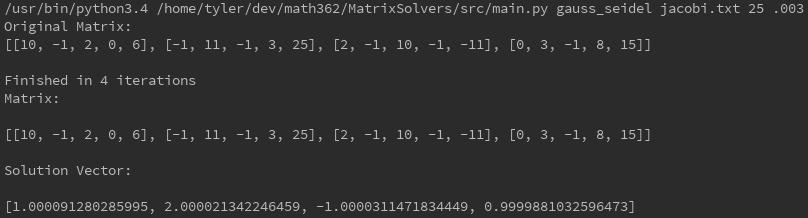
\includegraphics{gauss_seidel.png}
\caption{The Gauss-Seidel Method}
\label{gauss_seidel}
\end{figure}

Figure \ref{gauss_seidel} shows the usage of the Gauss-Seidel method. This method can be accessed by using ``gauss\_seidel''
as the solution method within the program.

\subsection{Successive Over-Relaxation Method}

The SOR method is a modification of the Gauss-Seidel method. The SOR method is 
an over-relaxtion method. This means that, by using some additional operations 
involving some constant $1 < \omega < 2$, we will converge faster. With a 
properly chosen $\omega$, convergence can be sped up greatly over the Gauss-Seidel
method. However, choosing an appropriate $\omega$ depends greatly on the matrix
itself. 

\begin{figure}[H]
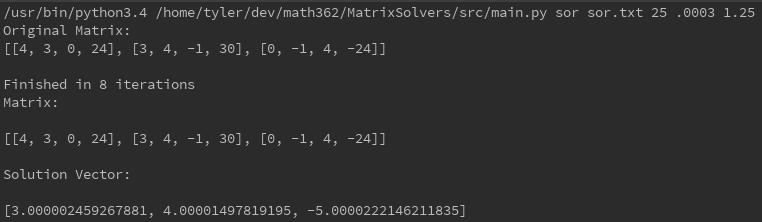
\includegraphics{sor.png}
\caption{The SOR Method}
\label{sor}
\end{figure}

\begin{figure}[H]
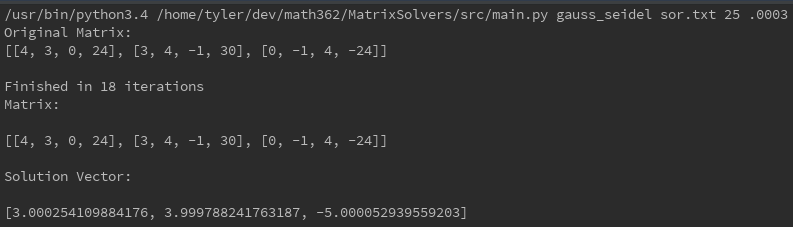
\includegraphics{slow_seidel.png}
\caption{The Gauss-Seidel Method}
\label{slow_seidel}
\end{figure}

Figure \ref{sor} shows the usage of the SOR method. In comparison to \figure{slow\_seidel},
it is apparent how a well chosen $\omega$ can have significant impact on the 
speed of convergence. This method can be accessed by using ``sor''
as the solution method within the program.



\section{Conclusion}
In conclusion, we have examined the implementation of 
 five algorithms for solving matrix equations: Gaussian Elimination, Gaussian Elimination with
Partial Pivoting, Jacobi's Method, The Gauss-Seidel Method, and a 
Successive Over-relaxation (SOR) Method. We have also looked at some example 
usage of this implementation. Future improvements to this work would include
adding additional solution methods, finding a way to calculate optimal values 
for some user-provided constants, such as $\omega$, adding consistency checks, 
and improving the matrix parsing algorithm.

\newpage

\end{document}
